\section{PDC Overview}
\subsection*{History}

\frame{
\frametitle{History of PDC}

\begin{itemize}
\item In 1988, envisioning that massive parallelism will become important for CS 
and HPC, a group of scientists from KTH School of Computer Science and 
Engineering applied for grant to buy a parallel computer
\item Market was surveyed and it was decided that Thinking Machines
Corporation (TMC) offered the best choice with its Connection Machine system, CM2
\item What was to be called the Center for Parallel Computers was formed and 
inaugurated by Janne Carlsson, the President of KTH, on January 15, 1990
\item In January 1991 PDC applied for an upgrade of the CM2 to a CM200. The
application was successful and the upgrade was installed in December 1991
\end{itemize}
}

\frame{
\frametitle{History of PDC}

\footnotesize
\begin{table}
  \begin{tabular}{r|r|r|r|l|l} \hline 
\textbf{Year} & \textbf{rank} & \textbf{procs.} & \textbf{peak gflops} & \textbf{vendor} & \textbf{name} \\ \hline
2011 &  31 & 36384 & 305626.00 & Cray & Lindgren\footnote{XE6 12-core 2.1 GHz} \\ \hline
2010 & 76 & 11016 & 92534.40 & Cray & Lindgren\footnote{XT6m 12-core 2.1 GHz} \\ \hline
2010 & 89 & 9800 & 86024.40 & Dell & Ekman\footnote{PowerEdge SC1435 Dual core Opteron 2.2GHz, Infiniband} \\ \hline
2005 & 65 & 886 & 5670.40 & Dell & Lenngren\footnote{PowerEdge 1850 3.2 GHz, Infiniband} \\ \hline
2003 & 196 & 180 & 648.00 & HP & Lucidor\footnote{Cluster Platform 6000 rx2600 Itanium2 900 MHz Cluster, Myrinet} \\ \hline
1998 & 60 & 146 & 93.44 & IBM & Strindberg\footnote{SP P2SC 160 MHz} \\ \hline
1996 & 64 & 96 & 17.17 & IBM & Strindberg\footnote{SP2/96} \\ \hline
1994 & 341 & 256 & 2.50 & Thinking Machines & Bellman\footnote{CM-200/8k} \\ \hline
  \end{tabular}
\end{table}

}

\subsection*{Member of SNIC}

\frame
{
\frametitle{SNIC}
\framesubtitle{Swedish National Infrastructure for Computing}
\begin{columns}
\column{.4\textwidth}
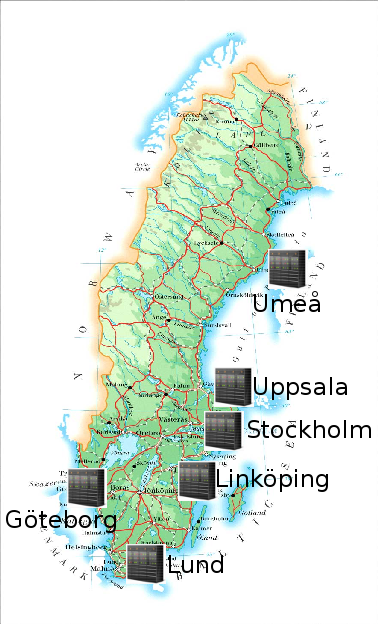
\includegraphics[width=0.8\linewidth]{sweden.png}\\
%\vspace{-55mm}
\column{.6\textwidth}
National \alert{research infrastructure} that provides a \alert{balanced and cost-efficient} set of \alert{resources and user support} for \alert{large scale computation and data storage} to meet the needs of researchers from all scientific disciplines and from all over Sweden (universities, university colleges, research institutes, etc).
\end{columns}
}



\subsection*{EU Access}
\frame{
\frametitle{Access to EU Facilities and Experts}
\begin{columns}
\column{.3\textwidth}

\includegraphics[width=0.9\linewidth]{eudat}\\~\\~\\~\\~\\

\includegraphics[width=0.9\linewidth]{epigram}
%\vspace{-55mm}
\column{.3\textwidth}

\includegraphics[width=0.9\linewidth]{prace}\\~\\

\includegraphics[width=0.9\linewidth]{egi}\\~\\

\includegraphics[width=0.9\linewidth]{einfra}


\column{.3\textwidth}

\includegraphics[width=0.9\linewidth]{cresta}\\

\includegraphics[width=0.9\linewidth]{7}

\end{columns}
}


\subsection*{Industry}
\frame{
\frametitle{PDC and Industry}
Working with industrial researchers and developers on major international projects that push high-performance computing to the next level. 
~\\~\\
Recently established a \alert{business development unit} that provides consultancy and HPC services to industries.
~\\~\\
\begin{columns}
\column{.25\textwidth}

\includegraphics[width=0.7\linewidth]{monotricat}
\column{.25\textwidth}

\includegraphics[width=0.9\linewidth]{ohb}
%\vspace{-55mm}
\column{.25\textwidth}

\includegraphics[width=0.9\linewidth]{pgs}
\column{.25\textwidth}

\includegraphics[width=0.9\linewidth]{scania}
\end{columns}

\begin{columns}
\column{.25\textwidth}

\includegraphics[width=0.7\linewidth]{logo_tyrens}
\column{.25\textwidth}

\includegraphics[width=0.9\linewidth]{fs_dynamics_logo}
\end{columns}

}


\subsection*{Training}
\frame{
\frametitle{Broad Range of Training}
\begin{description}
 \item [Summer School]  Introduction to HPC held every year
 \item [Specific Courses] Programming with GPGPU, Recent Advances in Distributed and Parallel Computing and/or Cloud Computing, Software Development Tools, etc
 \item [PDC User Days] PDC Pub and Open House
\end{description}

\begin{columns}
\column{.3\textwidth}
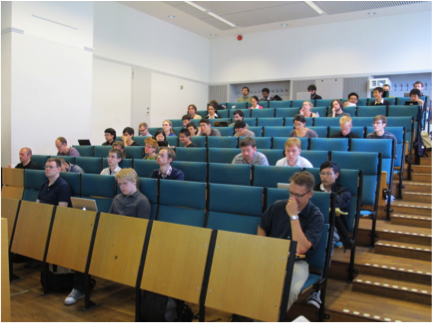
\includegraphics[width=0.9\linewidth]{class3}
\column{.3\textwidth}
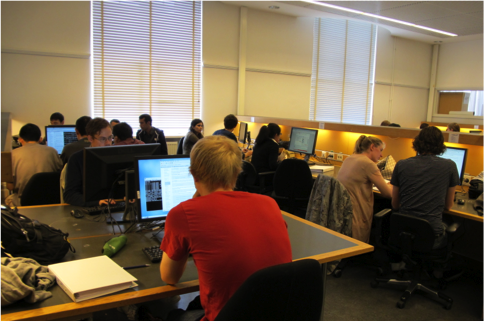
\includegraphics[width=0.9\linewidth]{class2}
\column{.3\textwidth}
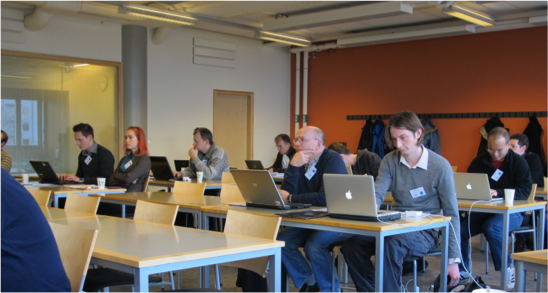
\includegraphics[width=0.9\linewidth]{class1}
\end{columns}
}

\subsection*{Staff}
\frame{
\frametitle{Support and System Staff}
\begin{exampleblock}{First-line support}
  Provide specific assistance to PDC users related to accounts, login, allocations etc.
\end{exampleblock}
\begin{exampleblock}{System staff}
  System managers/administrators ensure that computing and storage resources run smoothly and securely.
\end{exampleblock}
\begin{exampleblock}{Application Experts}
  Hold PhD degrees in various fields and specialize in HPC. Assist researchers in optimizing, scaling and enhancing scientific codes for current and next generation supercomputers.
\end{exampleblock}
}


\frame<presentation:0>[noframenumbering]{
\frametitle{Application Experts}
Hold PhD degrees in different scientific fields and are experts in HPC. Together with researchers, they optimize, scale and enhance scientific codes for the next generation supercomputers.
\footnotesize{
\begin{columns}

\column{.3\textwidth}
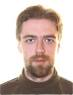
\includegraphics[width=0.5\linewidth]{jaime_rosal}\\ \textbf{Jaime Rosal Sandberg} \\ Computational Chemistry
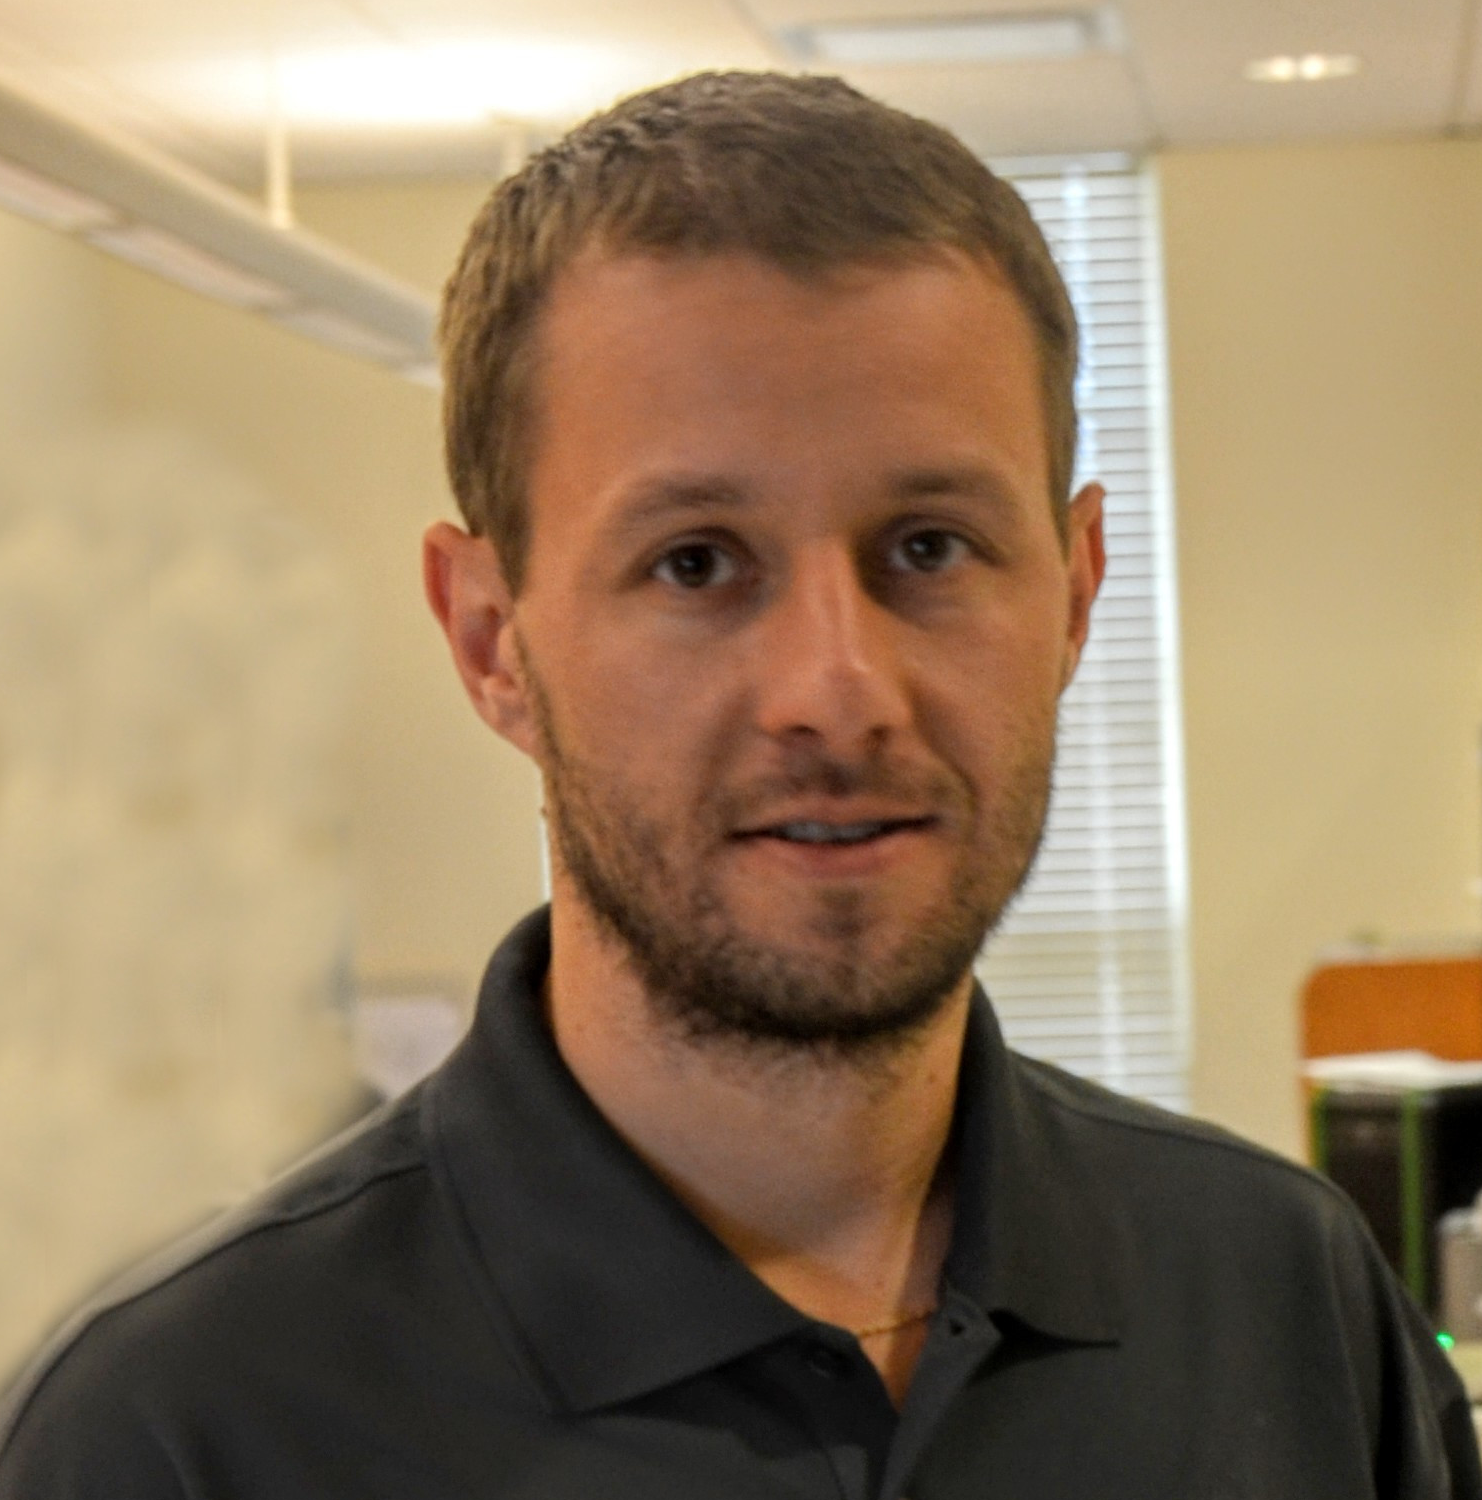
\includegraphics[width=0.5\linewidth]{cristian_cira}\\ \textbf{Cristian Cira}\\ Perfomance Analysis

\column{.3\textwidth}
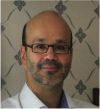
\includegraphics[width=0.5\linewidth]{henric_zazzi}\\ \textbf{Henric Zazzi}\\ Bioinformatics/Genetics
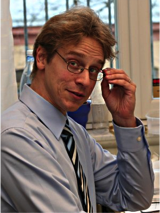
\includegraphics[width=0.5\linewidth]{michael_djurfeldt}\\ \textbf{Michael Djurfeldt}\\ Computational Physics

\column{.3\textwidth}
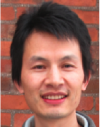
\includegraphics[width=0.5\linewidth]{jing_gong}\\ \textbf{Jing Gong} \\ Scientific Computing
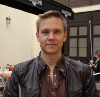
\includegraphics[width=0.5\linewidth]{thor_wikfeldt}\\ \textbf{Thor Wikfeldt} \\ Computational \\ Chemistry

\end{columns}
}}

\subsection*{Services}
\frame{
\frametitle{Services}
\begin{itemize}
\item Access to supercomputers
\item HPC training 
\item Postgraduate degree projects
\item Visualization
\item Support 
\item Expertise in HPC software
\item Access to international HPC facilities
\item Data storage
\end{itemize}
}
